\documentclass{article}

\usepackage[margin=1in]{geometry} 
\usepackage{amsmath,amsthm,amssymb,amsfonts, fancyhdr, color, comment, graphicx, environ,bbm}
\usepackage[dvipsnames]{xcolor}
\usepackage{subcaption}
\usepackage{mdframed}
\usepackage[shortlabels]{enumitem}
\usepackage{indentfirst}
\usepackage{hyperref}
\usepackage{placeins}
\usepackage{comment} %Comment large blocks
\usepackage{xfrac}
\usepackage{float} % To use "H" to force tables to be where wanted
\usepackage{booktabs} % Makes output from knittr:kable look better
\usepackage{parskip} %No indents for paragraphs
\usepackage[shortlabels]{enumitem} % To enumerate with letters
\hypersetup{
 colorlinks=true,
 linkcolor=blue,
 filecolor=magenta, 
 urlcolor=blue,
}
\pagestyle{fancy}
\usepackage{todonotes}

\newcommand{\E}{\mathbb{E}}
\renewcommand{\H}{\mathcal{H}}
\renewcommand{\L}{\mathcal{L}}
\newcommand{\dU}[1]{\ensuremath\frac{\partial u}{\partial #1}}
\newcommand{\dV}[1]{\ensuremath\frac{\partial v}{\partial #1}}
\newcommand{\ppx}[2]{\ensuremath\frac{\partial #1}{\partial #2}}
\newcommand{\ddx}[2]{\ensuremath\frac{d #1}{d #2}}
\newcommand{\indp}{\perp\!\!\!\perp} 

%\usepackage{mathpazo} %Dylan's fancy math bullshit that I don't want
\usepackage{microtype}
\usepackage{graphicx}
\usepackage{setspace}

%Footnote without a number
\newcommand\blfootnote[1]{%
  \renewcommand\thefootnote{}\footnote{#1}%
  \addtocounter{footnote}{-1}%
}

% Problem formatting [Alex]

\newenvironment{problem}[1]
    { \begin{mdframed}[backgroundcolor=Periwinkle!20] \textbf{(#1)} }
    {  \end{mdframed}}
% Define solution environment
\newenvironment{solution}{\textbf{Solution}\\}

%%%%%%%%%%%%%%%%%%%%%%%%%%%%%%%%%%%%%%%%%%%%%
%Fill in the appropriate information below
\lhead{Problem Set 1}
\rhead{Empirical Analysis} 
\title{Problem Set 2}
\author{Alex Weinberg \and Isaac Norwich \and Jose M. Quintero}

%%%%%%%%%%%%%%%%%%%%%%%%%%%%%%%%%%%%%%%%%%%%%
\begin{document}
\maketitle

Our code can be found in this GitHub respository: \url{https://github.com/jmquintero925/Metrics-III/tree/main/ps2}

%%%%%%%%%%%%%%%%%%%%%%%%%%%%%%%%%% QUESTION 1 %%%%%%%%%%%%%%%%%%%%%%%%%%%%%%%%%
\section*{Problem 1}
Let $Y_{i}(1)$ and $Y_{i}(0)$ be potential outcomes of individual $i$ if treated or not treated, respectively. Let $Y_{i}$ be the actual outcome and let $D_{i}$ be the treatment indicator. We assume:
\begin{align*}
\begin{gathered}
D_{i} \indp \left(Y_{i}(1), Y_{i}(0)\right) \mid X_{i} \\
0<P\left[D_{i}=1 \mid X_{i}=x\right]<1 \quad \forall x \in \operatorname{supp}\left(X_{i}\right)
\end{gathered}
\end{align*}

\begin{problem}{a}
Propose an estimator of $\E\left[Y_{i}(1)-Y_{i}(0)\right]$
\end{problem}
\begin{solution}
Begin by using the Law of iterated expectations note that the moment of interest can be rewritten as
\begin{align*}
    \E\left[Y_{i}(1)-Y_{i}(0)\right] &= \E\left[\E\left[Y_{i}(1)-Y_{i}(0)\big\vert X = x\right]\right] \\ 
    &= \E\left[\E\left[Y_{i}(1)\big\vert X_i = x\right]-\E\left[Y_{i}(0)\big\vert X_i = x\right]\right] \\ 
    &= \E\left[\E\left[Y_{i}(1)\big\vert X_i = x,D_i=1\right]-\E\left[Y_{i}(0)\big\vert X_i = x, D_i=0\right]\right] \\ 
    &= \E\left[\E\left[Y_{i}\big\vert X_i = x,D_i=1\right]-\E\left[Y_{i}\big\vert X_i = x, D_i=0\right]\right] \tag{ATE}\label{ps2:q1a:eq1}
\end{align*}
where the equality line uses the hypothesis $D_{i} \indp \left(Y_{i}(1), Y_{i}(0)\right) \mid X_{i}$ and the last equality uses the fact that $Y_i(1) = \left(Y_i\vert D_i=1\right)$. Next, conditional on $X_i=x$, the inside terms are averages that can be calculated straight from the data. Define the set 
\begin{equation*}
    I(d,x)=\{i\vert D_i=d\land X_i=x\}
\end{equation*}  as the set of individuals with treatment variable $d$ and observable $x$. Then $\E\left[Y_{i}\big\vert X = x,D_i=d\right]$ can be identified by 
\begin{equation*}
    \hat{\mu}(d,x) = \frac{1}{\vert I(d,x)\vert} \sum_{i\in I(d,x)} Y_i
\end{equation*} where $\vert\cdot\vert$ denotes the cardinality of the set. Thus a natural estimator for \eqref{ps2:q1a:eq1} is 
\begin{equation*}
    \widehat{\text{ATE}} = \int (\hat{\mu}(1,x)-\hat{\mu}(0,x))\mathrm{d}F(x)
\end{equation*}
Note that since $X_i$ is potentially a vector, the distribution is the joint density of each of the components of $X_i$. However, in practice, researchers only observe a finite set of values of $X_i$. Thus, one potential way of estimating the integral is 
\begin{equation*}
    \widehat{\text{ATE}} = \frac{1}{N}\sum_{x} (\hat{\mu}(1,x)-\hat{\mu}(0,x))(\vert I(1,x)\vert+\vert I(0,x)\vert)
\end{equation*}
\end{solution}

\begin{problem}{b}
Show that the assumptions stated imply that $D_{i}$ is conditionally independent of $\left(Y_{i}(1), Y_{i}(0)\right)$ given $P\left[D_{i}=1 \mid X_{i}\right]: D_{i} \indp\left(Y_{i}(1), Y_{i}(0)\right) \mid P\left[D_{i}=1 \mid X_{i}\right]$. Why is this result important?
\end{problem}
\begin{solution}
To show that $D_{i} \indp\left(Y_{i}(1), Y_{i}(0)\right) \mid P\left(D_{i}=1 \mid X_{i}\right)$ first define the propensity score $p(x)$ as 
\begin{equation*}
    p(x) = P(D_i=1\vert X_i=x).
\end{equation*}
Next, by Bayes rule
\begin{equation}\label{ps2:q1b:eq1}
    P\left(D_i=1\vert Y_i(1),Y_i(0),p(X_i)\right) = \frac{P\left(D_i=1, Y_i(1),Y_i(0)\vert p(X_i)\right)}{P\left(Y_i(1),Y_i(0)\vert p(X_i)\right)}
\end{equation}
By definition of independence, $D_{i} \indp\left(Y_{i}(1), Y_{i}(0)\right) \mid P\left(D_{i}=1 \mid X_{i}\right)$ if and only if 
\begin{equation}\label{ps2:q1b:eq2}
   P\left(D_i=1, Y_i(1),Y_i(0)\vert p(X_i)\right) =P\left(D_i=1\vert p(X_i)\right)P\left( Y_i(1),Y_i(0)\vert p(X_i)\right).
\end{equation}
Thus, by combining \eqref{ps2:q1b:eq1} and \eqref{ps2:q1b:eq2}, we I can conclude that $D_i$ is independent from $(Y_i(1),Y_i(0))$ is and only if the following condition holds:  
\begin{align*}
    P\left(D_i=1\vert Y_i(1),Y_i(0),p(X_i)\right) &= P\left(D_i=1\vert p(X_i)\right) \\ 
    &= p(X_i).
\end{align*}
Use the fact that $D_i$ is a binary variable and can be written in terms of expectations
\begin{align*}
    P\left(D_i=1\vert Y_i(1),Y_i(0),p(X_i)\right) &= \E\left[D_i\vert Y_i(1),Y_i(0),p(X_i) \right] \\ 
    &= \E\left[\E\left[D_i\vert Y_i(1),Y_i(0),X_i\right]\big\vert p(X_i) \right] \tag{LIE} \\ 
    &= \E\left[\E\left[D_i\vert X_i\right]\big\vert p(X_i) \right] \tag{CIA} \\ 
    &= \E\left[p(X_i) \big\vert p(X_i) \right] \\ 
    &= p(X_i)
\end{align*}
which is what we wanted to show. This result is very relevant because as shown in question (a) the dimension of $X_i$ can make the problem more imprecise. 
\end{solution}

\begin{problem}{c}
Define the propensity score $P\left[D_{i}=1 \mid X_{i}\right]$ as the probability of receiving the treatment given the observables variables $X_{i}$. Propose an estimator of $\E\left[Y_{i}(1)-Y_{i}(0)\right]$ based on the propensity score.
\end{problem}
\begin{solution}
We can emulate the estimator constructed in question (a) but now conditioning on $p(X_i)$: 
\begin{align*}
    \E\left[Y_{i}(1)-Y_{i}(0)\right] &= \E\left[\E\left[Y_{i}(1)-Y_{i}(0)\big\vert p(X_i) = p\right]\right] \\ 
    &= \E\left[\E\left[Y_{i}(1)\big\vert p(X_i) = p\right]-\E\left[Y_{i}(0)\big\vert p(X_i) = p\right]\right] \\ 
    &= \E\left[\E\left[Y_{i}(1)\big\vert p(X_i) = p,D_i=1\right]-\E\left[Y_{i}(0)\big\vert p(X_i) = p, D_i=0\right]\right] \\ 
    &= \E\left[\E\left[Y_{i}\big\vert p(X_i) = p,D_i=1\right]-\E\left[Y_{i}\big\vert p(X_i) = p, D_i=0\right]\right]
\end{align*}
Thus, as before we can create the mean of the outcome conditional on the propensity score
\begin{equation*}
     \hat{\mu}(d,p) = \frac{1}{\vert I(d,p)\vert} \sum_{i\in I(d,p)} Y_i
\end{equation*}
where the set $I$ is defined similarly to the one in question (a) but instead of conditioning on the observable variables is conditioning on the propensity score. Then an estimator for the ATE
\begin{align*}
\widehat{\text{ATE}} = \int \left(\mu(1,p)-\mu(0,p)\right)\mathrm{d}F(p)
\end{align*}
Empirically, since the pscore is a continuous variable, one can always create bins and box all observations such that the pscore lands in the same bin. This is somehow arbitrary as the size of the bin is a free variable. 
\end{solution}

\newpage
%%%%%%%%%%%%%%%%%%%%%%%%%%%%%%%%%% QUESTION 2 %%%%%%%%%%%%%%%%%%%%%%%%%%%%%%%%%
\section*{Problem 2}
LaLonde (AER, 1986) investigated whether non-experimental methods could reproduce the experimental estimate based on the National Supported Work (NSW) Demonstration. The following dataset from Smith and Todd (J Ectrics, 2005):
\begin{center}
    \hyperlink{https://www.dropbox.com/s/dl/aw4yi13mz9z03yf/lalonde2.dta}{https://www.dropbox.com/s/dl/aw4yi13mz9z03yf/lalonde2.dta}
\end{center}
includes the NSW sample, as well as two non-experimental samples: one based on the Current Population Survey (CPS) and one on the Michigan Panel of Income Dynamics (PSID). The variable -sample- identifies the relevant observations. The variable -treated- identifies the observations that were treated (participate in a subsidized work experience program) in the NSW (from April 1975 to August 1977). You are interested in the average effect on Real Earnings in 1978 of the treatment for the treated. Start with the NSW sample:
\begin{problem}{a}
Investigate whether the data is consistent with randomization of the treatment.
\end{problem}
\begin{solution}
To check if the sample is consistent with randomization, we calculate the mean difference between the control variables. The results are presented in Table \ref{ps2:q2a:tab1}
\begin{table}[htb]
    \centering
    \caption{Randomization}
    \label{ps2:q2a:tab1}
    {
\def\sym#1{\ifmmode^{#1}\else\(^{#1}\)\fi}
\begin{tabular}{l*{3}{cccc}}
\hline\hline
                    &\multicolumn{2}{c}{(1)}  &\multicolumn{2}{c}{(2)}  &\multicolumn{2}{c}{(3)}           \\
                    &\multicolumn{2}{c}{Treated}&\multicolumn{2}{c}{Untreated}&\multicolumn{2}{c}{Mean Difference}\\
                    &        mean&          sd&        mean&          sd&           b         &           t\\
\hline
age of individual   &      24.626&       6.686&      24.447&       6.590&      -0.179         &    (-0.357)\\
years of schooling  &      10.380&       1.818&      10.188&       1.619&      -0.192         &    (-1.492)\\
1 if Black, 0 otherwise&       0.801&       0.400&       0.800&       0.400&      -0.001         &    (-0.045)\\
1 if married, 0 otherwise&       0.168&       0.375&       0.158&       0.365&      -0.011         &    (-0.384)\\
1 if High School dropout, 0 otherwise&       0.731&       0.444&       0.814&       0.389&       0.083\sym{**} &     (2.673)\\
1 if Hispanic, 0 otherwise&       0.094&       0.293&       0.113&       0.317&       0.019         &     (0.803)\\
# kids younger than 18&       0.343&       0.844&       0.313&       0.854&      -0.030         &    (-0.474)\\
kidmiss             &       0.101&       0.302&       0.127&       0.333&       0.026         &     (1.074)\\
Real Earnings 1974  &    3570.999&    5773.134&    3672.485&    6521.526&     101.486         &     (0.216)\\
\hline
Observations        &         297&            &         425&            &         722         &            \\
\hline\hline
\end{tabular}
}

\end{table}
Note that there is no statistical difference in the mean of the control variables that suggest some selection going on with the exception of High school drop out. 


\end{solution}

\begin{problem}{b}
Estimate the effect using the experimental sample. Now use the sample consisting in the treated from the NSW sample and the comparison individuals from the CPS sample.
\end{problem}
\begin{solution}
Since the treatment is randomize, we can do a difference of means to calculate the ATE/ATT/ATUT. The results are presented in Table \ref{ps2:q2b:tab1}
\begin{table}[htb]
    \centering
    \caption{ATE}
    \label{ps2:q2b:tab1}
    {
\def\sym#1{\ifmmode^{#1}\else\(^{#1}\)\fi}
\begin{tabular}{l*{3}{cccc}}
\hline\hline
                    &\multicolumn{2}{c}{(1)}  &\multicolumn{2}{c}{(2)}  &\multicolumn{2}{c}{(3)}           \\
                    &\multicolumn{2}{c}{Treated}&\multicolumn{2}{c}{Untreated}&\multicolumn{2}{c}{ATE}           \\
                    &        mean&          sd&        mean&          sd&           b         &           t\\
\hline
Real Earnings 1978  &    5976.352&    6923.796&    5090.048&    5718.089&    -886.304         &    (-1.877)\\
\hline
Observations        &         297&            &         425&            &         722         &            \\
\hline\hline
\end{tabular}
}

\end{table}
This is equivalent to run a regression on the outcome and the treatment variable. 
\end{solution}

\begin{problem}{c}
Estimate the effect using OLS.
\end{problem}
\begin{solution}
\begin{table}[htb]
    \centering
    \caption{Effect using OLS}
    \label{tab:my_label}
    \begin{tabular}{lcc} \hline\hline
 & (1) & (2) \\
Variables & \multicolumn{2}{c}{Real Earnings 78} \\ \hline 
D & -8,870.308*** & -1,568.938*** \\
 & (562.478) & (474.716) \\
 &  &  \\ \hline
Observations & 16,289 & 16,289 \\
R-squared & 0.015 & 0.428 \\
 Controls & No & Yes \\ \hline\hline
\multicolumn{3}{c}{ Standard errors in parentheses} \\
\multicolumn{3}{c}{ *** p$<$0.01, ** p$<$0.05, * p$<$0.1} \\
\end{tabular}

\end{table}
\end{solution}

\begin{problem}{d}
Investigate covariate balancing and support between the treated and the CPS sample.
\end{problem}
\begin{solution}
To investigate the balancing of covariates we can repeat the exercise in question (a). The results are presented in Table \ref{ps2:q2d:tab1}. Unlike question (a), there are several differences in the mean which are statistically significant and thus we can no longer conclude that there is randomization without selection on the covariates. 
\begin{table}[htb]
    \centering
    \caption{Covariate Balancing}
    \label{ps2:q2d:tab1}
 {
\def\sym#1{\ifmmode^{#1}\else\(^{#1}\)\fi}
\begin{tabular}{l*{3}{cccc}}
\hline\hline
                    &\multicolumn{2}{c}{(1)}  &\multicolumn{2}{c}{(2)}  &\multicolumn{2}{c}{(3)}           \\
                    &\multicolumn{2}{c}{Treated}&\multicolumn{2}{c}{Untreated}&\multicolumn{2}{c}{Mean Difference}\\
                    & Mean & SD & Mean & SD & Estimate & $t$-value \\
\hline
Age   &      24.626&       6.686&      33.225&      11.045&       8.599\sym{***}&    (13.371)\\
Schooling  &      10.380&       1.818&      12.028&       2.871&       1.647\sym{***}&     (9.850)\\
Black &       0.801&       0.400&       0.074&       0.261&      -0.728\sym{***}&   (-47.041)\\
Married &       0.168&       0.375&       0.712&       0.453&       0.543\sym{***}&    (20.543)\\
High School dropout &       0.731&       0.444&       0.296&       0.456&      -0.435\sym{***}&   (-16.274)\\
Hispanic &       0.094&       0.293&       0.072&       0.259&      -0.022         &    (-1.465)\\
\# Kids younger than 18&       0.343&       0.844&       1.834&       1.695&       1.491\sym{***}&    (15.122)\\
kidmiss             &       0.101&       0.302&       0.004&       0.064&      -0.097\sym{***}&   (-21.929)\\
Real Earnings 1974  &    3570.999&    5773.134&   14016.801&    9569.796&   10445.802\sym{***}&    (18.748)\\
\hline
Observations        & \multicolumn{2}{c}{297}&\multicolumn{2}{c}{15992}&\multicolumn{2}{c}{16289} \\
\hline\hline
\end{tabular}
}

\end{table}
Furthermore, the support between both groups on the continuous covariates are presented Figure \ref{ps2:q2d:fig1}. Binary variables are not necesary to plot as long as their mean in Table \ref{ps2:q2d:tab1} is not exactly 0 or 1 (which is not the case). 
\begin{figure}[htb]
    \centering
    \caption{Covariate Balancing}
    \label{ps2:q2d:fig1}
    \begin{subfigure}[b]{0.4\textwidth}
         \centering
         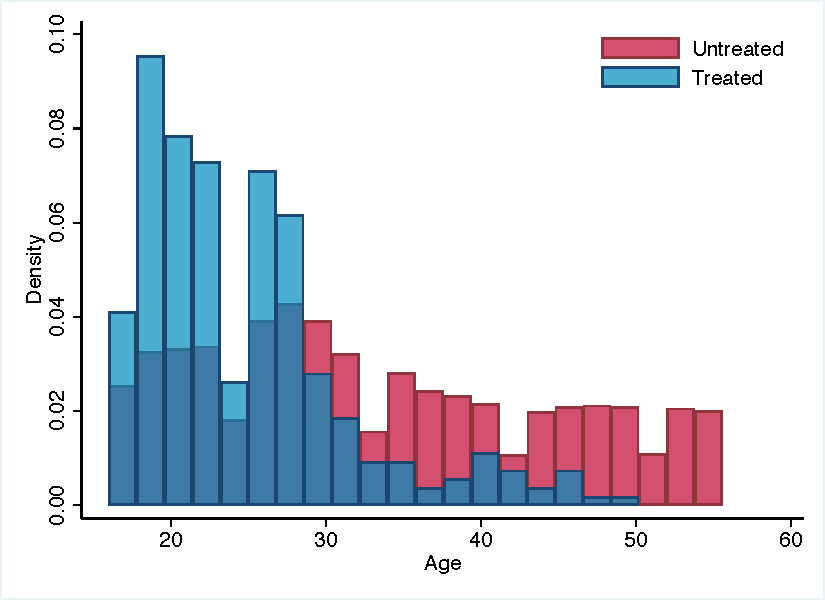
\includegraphics[width=\textwidth]{ps2/Figures/ps2_q2d_age.pdf}
         \caption{Age}
     \end{subfigure}
     \begin{subfigure}[b]{0.4\textwidth}
         \centering
         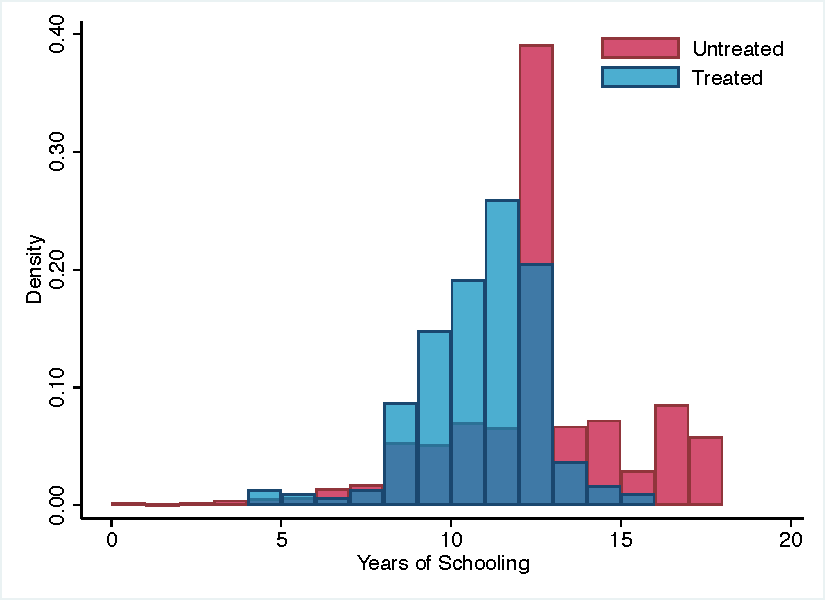
\includegraphics[width=\textwidth]{ps2/Figures/ps2_q2d_educ.pdf}
         \caption{Schooling}
     \end{subfigure}
     \hfill
     \begin{subfigure}[b]{0.4\textwidth}
         \centering
         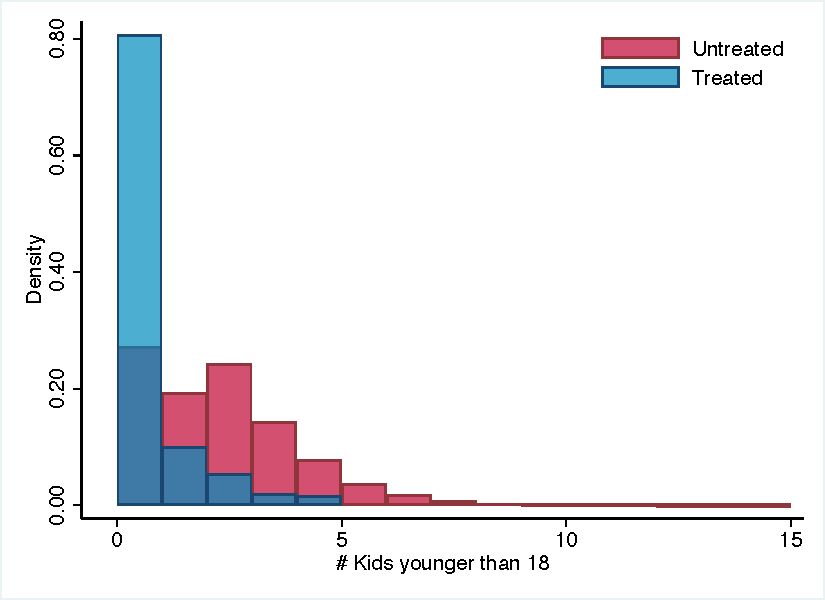
\includegraphics[width=\textwidth]{ps2/Figures/ps2_q2d_kids18.pdf}
         \caption{\# Kids under 18}
     \end{subfigure}
     \begin{subfigure}[b]{0.4\textwidth}
         \centering
         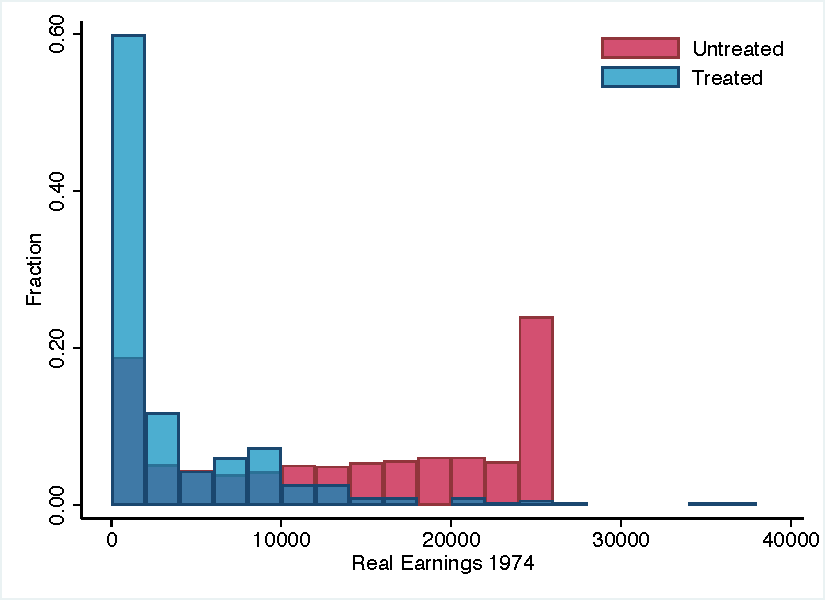
\includegraphics[width=\textwidth]{ps2/Figures/ps2_q2d_re74.pdf}
         \caption{Real Earnings 74}
         \label{fig:lab_prod}
     \end{subfigure}
\end{figure}

Finally, we present the common support on the propensity score calculated using a probit regression. 
\begin{figure}
    \centering
    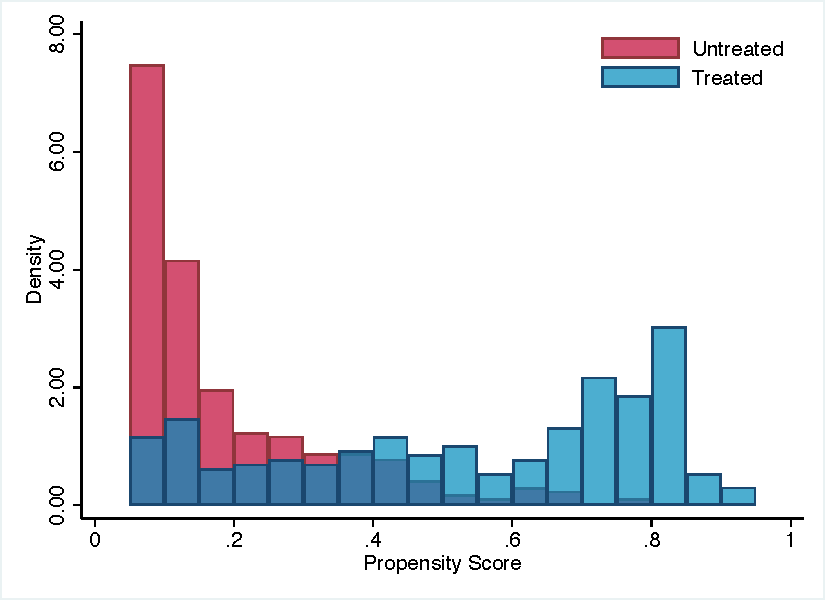
\includegraphics[width=0.45\textwidth]{ps2/Figures/ps2_q2d_pscore.pdf}
    \caption{Propensity Score}
\end{figure}
\end{solution}
\FloatBarrier
\begin{problem}{e}
Estimate the effect using 1 nearest neighbor propensity score matching. (Use -psmatch2- which can be installed using: ssc install psmatch2, if you use Stata. Other languages have
similar programs.).
\end{problem}
\begin{solution}
We use psmatch2 to find a good control for every treated observation and calculate the ATT. We do not report standard errors as the function in Stata does not account for the ``first stage''. 
\begin{table}[htb]
    \centering
    \caption{Treatment on the Treated}
    \label{tab:my_label}
    \begin{tabular}{lcc} \hline\hline 
 & (1) & (2) \\ \\ \hline
     ATT & -413.09 & -697.77  \\ \hline
     Controls & No & Yes \\ \hline\hline
\end{tabular}
\end{table}

\end{solution}

\begin{problem}{f}
Estimate the effect using the propensity score and local linear regression.
\end{problem}
\begin{solution}
The ATT using a local linear regression of degree 1 and a rectangular kernel is  -516.59. See the details in the attached code. 
\end{solution}

\newpage
%%%%%%%%%%%%%%%%%%%%%%%%%%%%%%%%%% QUESTION 3 %%%%%%%%%%%%%%%%%%%%%%%%%%%%%%%%%
\section*{Problem 3}
You are interested in estimating the effect of doing mathematics homework (yes/no) on mathematics test scores. You have data on all 10th graders in Oslo for the school year 2010/2011. The dataset contains the following variables:
\begin{itemize}
    \item students: end year test scores, homework, of missed classes, gender, age, test scores in 2009/2010
    \item parents: education
    \item teacher: gender, age, education
\end{itemize}
About half of the students do their homework.

\begin{problem}{a}
If you want to abolish homework, what effect would you want to estimate?
\end{problem}
\begin{solution}
If you want to abolish homework, the policy you want to impose is $D=0$ for all students. You would want to show that doing so would not harm the outcome of students who currently are doing their homework when you no longer give them homework to do. That is, we want to estimate the average treatment effect on the treated (ATT) and see if it is 0. The ATT is the amount by which students who currently do their homework benefit, so it will be that amount by which their end of year test scores go down if homework is abolished. The ATT formula is $E[Y_1-Y_0|D=1]$.
\end{solution}

\begin{problem}{b}
If you want to make homework mandatory, what effect would you want to estimate?
\end{problem}
\begin{solution}
If you want to make homework mandatory, you would want to know the effect of treatment (homework) on the untreated, ATUT. That is, we want to know what would the impact of making homework mandatory be on the outcomes for the subset of people who currently do not do their homework. The ATUT is $E[Y_1-Y_0|D=0]$. 
\end{solution}

\begin{problem}{c}
You want to compare the effect of doing homework as compared to an extra hour of math teaching. What effect of homework would you like to know?
\end{problem}
\begin{solution}
To compare the effect of doing homework as compared to an extra hour of math teaching, we would want to know the ATE. The ATE is the average effect of doing homework for all 10th graders in Oslo, regardless of whether they are currently doing homework or not. The ATE is $E[Y_1-Y_0]$. We would then compare this effect to the effect of an extra hour of math teaching.\todo[inline]{Uhhh how do we get the effect of an hour of math teaching effect?? Or is that irrelevant to the answer?}
\end{solution}

\textbf{You want to estimate how well students that are currently not doing their homework would do, if they did their homework. You decide to use matching, and will therefore rely on a conditional independence assumption (CIA).}
\begin{problem}{d}
Explain your CIA. Be explicit about the counterfactual outcomes and the variables that you want to control for. Why might your CIA not hold? Can you think of examples where you get upward biased estimates? And downward biased estimates?
\end{problem}
\begin{solution}
We want to estimate the average treatment effect on the untreated: $\operatorname{ATUT} = E[Y_1|D=0]-E[Y_0|D=0]$. This estimate will tell us how well students who are not doing their homework ($D=0$) \textit{would} do if they did their homework ($Y_1$) compared to how they do now ($Y_0$).

The conditional independence assumption is that the potential outcomes are independent of treatment, conditional on covariates: $(Y_0,Y_1)\perp D | X$. In this case, our potential outcomes are the end of year test scores for a student who does ($Y_1$) and does not do ($Y_0$) their homework ($D$). 

The variables we want to control for, $X$, are those that will impact selection into treatment, so that conditioning on them allows us to view the treatment of doing homework as random across individuals. To do so, we must only control for observables that are determined before treatment.  Given the rich data, we would want to include all covariates except for our outcome (``end year test scores'') and the number of missed classes, since this is clearly not a predetermined variable. Everything else will be useful for our CIA.
    
The CIA might not hold if there are other variables that impact selection into doing or not doing homework. Since we are estimating the impact of math homework on end of year test scores, we could be omitting a measure of taste for mathematics. Certain students, even though they are good at math, may dislike math and therefore not do their math homework. If two students are perfectly matched on $X$'s except for this omitted `taste' measure, then treatment of doing homework will not be random since the one who likes math will be more likely to select into treatment. This would break our CIA.

We would get upward biased estimates if the covariance between the omitted variable and the included variables (in the short regression) is positive. Specifically, if treatment (doing homework, $D$), is positively correlated with taste for mathematics, then the estimate from a regression without this variable would be upwardly biased. If the correlation is negative, then we would get downward biased estimated. This could happen if students who do not like math think that doing the homework will help them do better on the end of year tests and thus, and thus the correlation between $D$ and taste for math is negative.
\end{solution}

\begin{problem}{e}
Explain how you use the CIA to estimate the counterfactual outcome, how you take into account that students that do their homework have different characteristics, and what support condition you need
\end{problem}
\begin{solution}
The counterfactual outcome we want to estimate is the effect of doing homework ($Y_1$) for students who do not currently do their homework ($D=0$): $E[Y_1|D=0]$. Note that this is the first part of the ATUT, and is all we need to estimate that effect, since $E[Y_0|D=0]$ is observed in the data.

To estimate this counterfactual outcome we must condition on covariates so that we can use the actual outcome of students who did their homework with the same covariate values as those that didn't. To do so, we use the CIA which tells us that expected outcomes for individuals with covariates $X$ are the same whether they received treatment or not: $E[Y_1|X,D=0]=E[Y_1|X,D=1]$.

To do so, start with the counterfactual outcome we want to find:
\begin{align}
    E[Y_1|D=0] &= E_X[ E[Y_1| X=x, D=0] | D=0] \tag{Expand inside using LIE} \\
    &=E_X[ E[Y_1| X=x, D=1] | D=0] \tag{Use CIA} \\
    &= \sum_{x} E[Y_1 | X=x, D=1] P(X=x|D=0) \tag{$E_X[\cdot]$ as weighted sum}
\end{align}

The last line shows the importance of the support condition. In order to properly match individuals, we need both treated and control observations for every combination of covariate values possible. For any $x^\star$ in the data, can't have $P(X=x^\star|D=0)$ be equal to either 1 or 0, otherwise that means that for all individuals with $X=x^\star$, they are either all treated or all not treated, which means we have no one to match them to. If this is the case, then the counterfactual that we are estimating will not include information from people with $X=x^\star$ and thus is not relevant to our sample, just a portion of it.

We have taken in to account the fact that students that do their homework may have different characteristics from those that do not. For instance, students with parents who have higher education levels may be more likely to do their homework. However, if we match students with parents who have the same level of education then we can estimate the impact of doing your homework on outcome. This is the CIA in action!

\end{solution}

\begin{problem}{f}
How would you estimate your effect using OLS?
\end{problem}
\begin{solution}
To estimate the effect (ATUT) using OLS, we want to construct an estimate of the mean comparison within each group $X=x$ and then weight these comparisons using the ATUT matching weight:
\begin{align*}
    \delta_x &\equiv E[Y_1|X,D=1]-E[Y_0|X,D=0] \\
    p(X) &\equiv P(D=1|X) \\
    w_{x,ATUT} &= (1-p(X))P(X=x) \\
    \implies \operatorname{ATUT} &= E[\delta_x | D=0] \\
    &= \frac{\sum_x \delta_x w_{x,ATUT}}{\sum_x w_{x,ATUT}}
\end{align*}

First, to obtain the mean comparison $\delta_x$, we use OLS and run:
\begin{align*}
    Y = \sum_x \delta_x \mathbf{1}[X=x] + \varepsilon
\end{align*}

Now, to compute the weight, we can 

\todo[inline]{Much easier to just do it for the counterfactual and then subtract out the part we see in the data ya dummy}

Using OLS, we would run a saturated-in-$X$ regression with a dummy for treatment versus control:\footnote{See MHE Eq 3.3.4 and Slide 26 of Topic2.pdf}


\end{solution}


\begin{problem}{g}
You see in your data that boys never do their homework. What implications does this have for your research?
\end{problem}
\begin{solution}
If boys never do their homework, then the common support assumption does not hold. Any cell that includes boys will be not treated and any cell that includes girls will be treated. Thus we cannot make comparisons within cells, since each cell will have all observations either treated or untreated. 
\todo[inline]{Conroy says something about getting an effect for girls, but I don't understand how}
\end{solution}

\textbf{You discover that not all teachers assign homework, and you get a new variable from Oslo municipality with information $(0 / 1)$ on whether the teacher assigned homework or not. They tell you that teachers were assigned to give homework (or not) in a randomized experiment.}
\begin{problem}{h}
First you add this new information to your matching variables. What will happen to your estimates and standard errors?
\end{problem}
\begin{solution}
If we add this new information to our matching variables, the estimates will not be impacted because this new variable is randomly assigned and thus has no correlation with any of the other covariates. The standard errors will increase, because we have now increased the dimensionality. For all observations, half now have had a teacher that was assigned to give homework or not randomly. Thus, in expectation, each cell of size $n$ now is reduced to size $\frac{n}{2}$ since half of the previous cell is randomly assigned the value $0$ or $1$ for this new variable. With the smaller cell size, our standard errors increase.
\end{solution}


\begin{problem}{i}
How will you use this new data and what effects can you estimate?
\end{problem}
\begin{solution}
LATE!
\end{solution}


\newpage
%%%%%%%%%%%%%%%%%%%%%%%%%%%%%%%%%% QUESTION 4 %%%%%%%%%%%%%%%%%%%%%%%%%%%%%%%%%
\section*{Problem 4}
Setup text here

\begin{problem}{a}
Plot a histogram of the data
\end{problem}
\begin{solution}
\begin{figure}[!htb]
    \centering    
    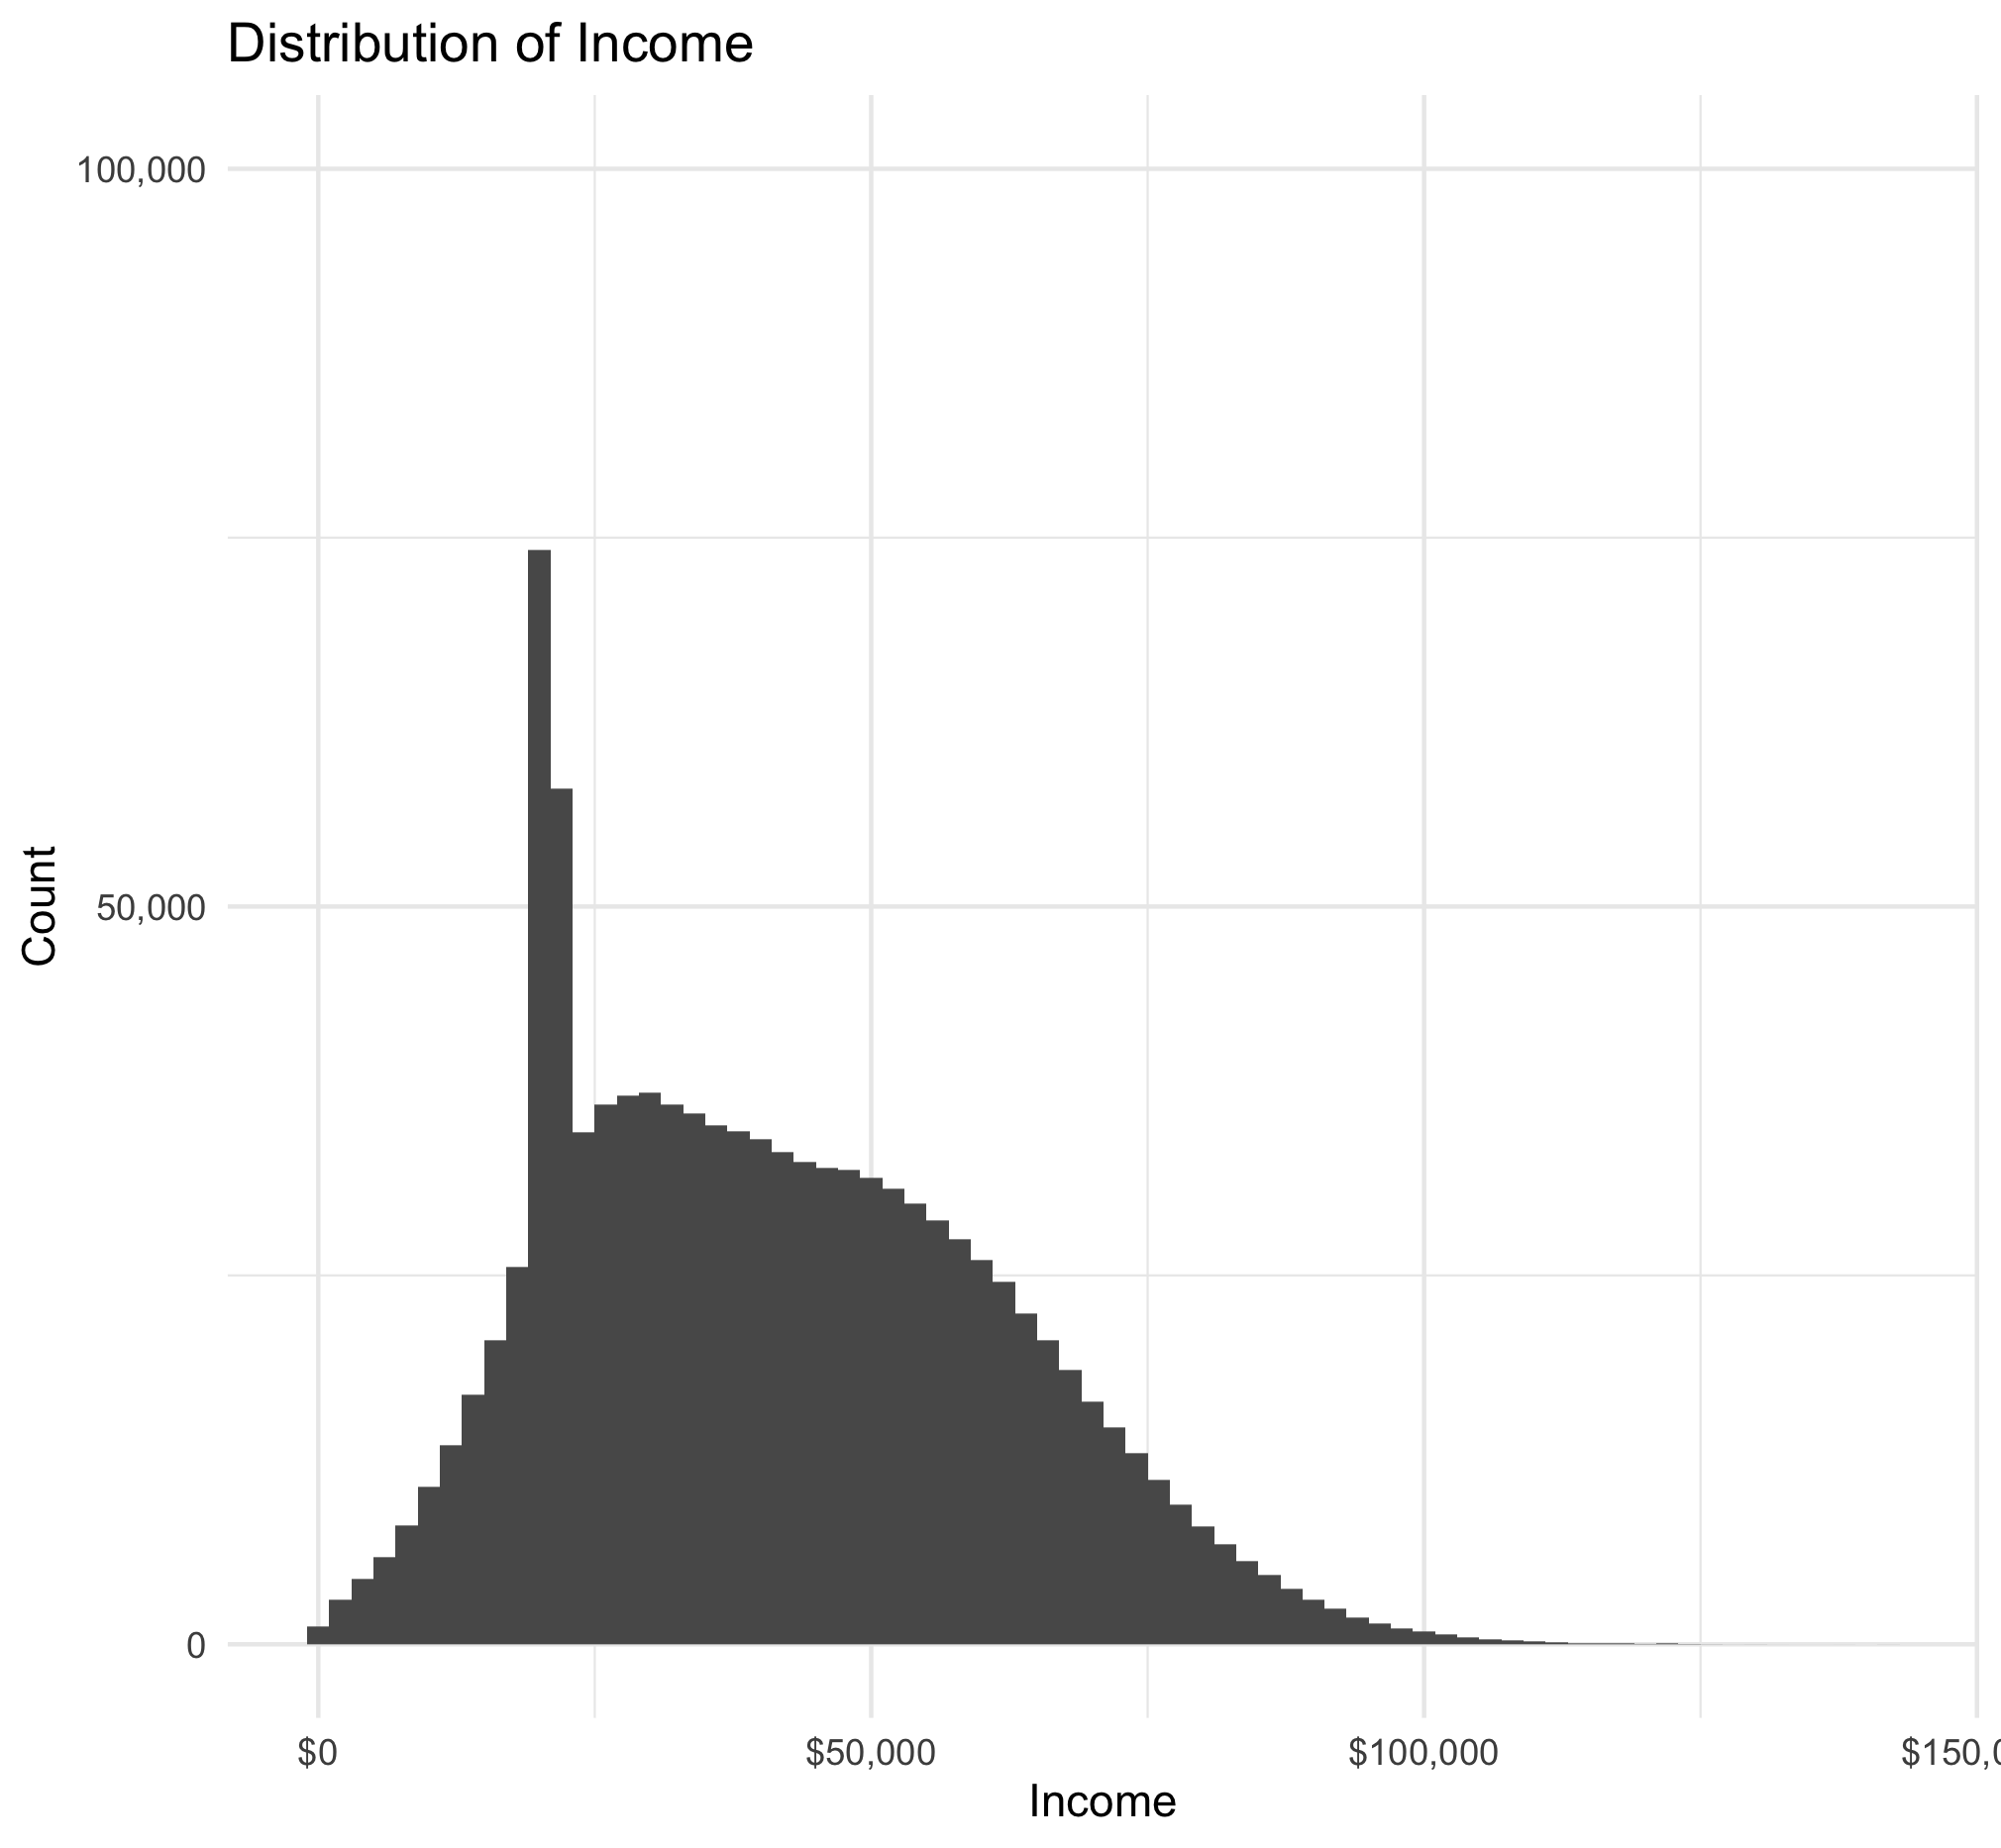
\includegraphics[width=0.75\textwidth]{ps2/4a.png}
\end{figure}

\end{solution}

\begin{problem}{b}
Compute estimates for f-(18000) and f+(22000) and bunching probability PK.
\end{problem}
\begin{solution}
I use a non-parametric estimator. Recall that the excluded range is given by the bounds
\begin{align*}
    y_1 &= K - \delta = 18000 \\
    y_2 &= K + \delta = 22000
\end{align*}

Count the number of data points in a band near the exluded range bounds. 
\begin{align*}
    N_1 &= \sum 1_{y\in [y_1-\delta, y_1]} \\
    N_2 &= \sum 1_{y\in [y_2, y_2+\delta]}
\end{align*}

I simply estimate non-parametrically 
\begin{align*}
    f^-(18000) &= \frac{N_1}{N} \\
    f^+(22000) &= \frac{N_2}{N}
\end{align*}

The implied data PK is of course

$$
\widehat{P}_K = \frac{\sum 1_{y\in [y_1, y_2]}}{N} - \delta * [f^-(18000) + f^+(22000)]
$$

In this data I find that

\begin{table}[h]
    \centering
    \begin{tabular}{c|c}
    \begin{array}{lll}
    \hline f^{-}(18000) & f^{+}(22000) & P_{K} \\
    \hline 0.0000106 & 0.000016 & 0.0687564 \\
    \hline
    \end{array}
    \end{tabular}
    \caption{Estimates}
    \label{tab:my_label}
\end{table}

\end{solution}

\begin{problem}{c}
Given density, compute elasticity.
\end{problem}
\begin{solution}
From equation 6 of the Blomquist et. al. paper we know that 
\[
P_{K}=\int_{\eta_{\ell}}^{\eta_{u}}\phi(\eta)d\eta
\]

Now our task is to identify $\beta$, the elasticity. To do so, we
will write $P_{K}$ as a function of both our density $\phi$ and
our elasticity $\beta$. Since $P_{K}$ is pinned down by the data
and $\phi$ is pinned down by our assumption, we will recover $\beta$. 

\paragraph{First specification.
\[
\ensuremath{\phi(\eta)=\phi\left(\eta_{1}\right)+\frac{\eta-\eta_{1}}{\eta_{2}-\eta_{1}}\left(\phi\left(\eta_{2}\right)-\phi\left(\eta_{1}\right)\right),\eta\in\left[\eta_{1},\eta_{2}\right]}
\]
}

\begin{align*}
P_{K} & =\int_{\eta_{\ell}}^{\eta_{u}}\phi(\eta)d\eta\\
 & =\int_{\eta_{\ell}}^{\eta_{u}}\phi\left(\eta_{1}\right)+\frac{\eta-\eta_{1}}{\eta_{2}-\eta_{1}}\left(\phi\left(\eta_{2}\right)-\phi\left(\eta_{1}\right)\right)d\eta\\
 & =\int_{\eta_{\ell}}^{\eta_{u}}\phi\left(\eta_{1}\right)-\frac{\eta_{1}}{\eta_{2}-\eta_{1}}\left(\phi\left(\eta_{2}\right)-\phi\left(\eta_{1}\right)\right)d\eta+\frac{\left(\phi\left(\eta_{2}\right)-\phi\left(\eta_{1}\right)\right)}{\eta_{2}-\eta_{1}}\int_{\eta_{\ell}}^{\eta_{u}}\eta d\eta\\
 & =\left[\phi\left(\eta_{1}\right)-\frac{\eta_{1}}{\eta_{2}-\eta_{1}}\left(\phi\left(\eta_{2}\right)-\phi\left(\eta_{1}\right)\right)\right]\left(\eta_{2}-\eta_{1}\right)+\frac{\left(\phi\left(\eta_{2}\right)-\phi\left(\eta_{1}\right)\right)}{\eta_{2}-\eta_{1}}\frac{\eta_{2}^{2}-\eta_{1}^{2}}{2}\\
 & =\left[\eta_{2}\phi\left(\eta_{1}\right)-\eta_{1}\phi\left(\eta_{2}\right)\right]+\frac{\left(\phi\left(\eta_{2}\right)-\phi\left(\eta_{1}\right)\right)}{\eta_{2}-\eta_{1}}\frac{\eta_{2}^{2}-\eta_{1}^{2}}{2}\\
 & =\left[\eta_{2}\phi\left(\eta_{1}\right)-\eta_{1}\phi\left(\eta_{2}\right)\right]+\frac{\phi\left(\eta_{2}\right)-\phi\left(\eta_{1}\right)}{\eta_{2}-\eta_{1}}\frac{\left(\eta_{2}-\eta_{1}\right)\left(\eta_{2}+\eta_{1}\right)}{2}\\
 & =\left[\eta_{2}\phi\left(\eta_{1}\right)-\eta_{1}\phi\left(\eta_{2}\right)\right]+\frac{\left(\phi\left(\eta_{2}\right)-\phi\left(\eta_{1}\right)\right)\left(\eta_{2}+\eta_{1}\right)}{2}\\
 & =\eta_{2}\phi\left(\eta_{1}\right)-\eta_{1}\phi\left(\eta_{2}\right)+\frac{\eta_{2}\phi\left(\eta_{2}\right)-\eta_{2}\phi\left(\eta_{1}\right)+\eta_{1}\phi\left(\eta_{2}\right)-\eta_{1}\phi\left(\eta_{1}\right)}{2}\\
 & =\frac{1}{2}\eta_{2}\phi\left(\eta_{1}\right)-\frac{1}{2}\eta_{1}\phi\left(\eta_{2}\right)+\frac{1}{2}\eta_{2}\phi\left(\eta_{2}\right)-\frac{1}{2}\eta_{1}\phi\left(\eta_{1}\right)\\
 & =\frac{1}{2}\left(\eta_{2}-\eta_{1}\right)\phi\left(\eta_{1}\right)+\frac{1}{2}\left(\eta_{2}-\eta_{1}\right)\phi\left(\eta_{2}\right)\\
 & =\frac{1}{2}\left(\eta_{2}-\eta_{1}\right)\left[\phi\left(\eta_{1}\right)+\phi\left(\eta_{2}\right)\right]
\end{align*}


\paragraph{Second specification}

\[
\ensuremath{\phi(\eta)=\begin{cases}
\phi\left(\eta_{1}\right) & ,\eta\in\left[\eta_{1},\frac{1}{4}\eta_{1}+\frac{3}{4}\eta_{2}\right]\\
\phi\left(\eta_{1}\right)+\frac{\eta-\left(\frac{1}{4}\eta_{1}+\frac{3}{4}\eta_{2}\right)}{\eta_{2}-\left(\frac{1}{4}\eta_{1}+\frac{3}{4}\eta_{2}\right)}\left(\phi\left(\eta_{2}\right)-\phi\left(\eta_{1}\right)\right) & ,\eta\in\left(\frac{1}{4}\eta_{1}+\frac{3}{4}\eta_{2},\eta_{2}\right]
\end{cases}}
\]

So then the integral is (I omit the algebra)

\[
\begin{aligned}P_{K} & =\int_{\eta_{1}}^{\frac{1}{4}\eta_{1}+\frac{3}{4}\eta_{2}}\phi\left(\eta_{1}\right)\mathrm{d}\eta+\int_{\frac{1}{4}\eta_{1}+\frac{3}{4}\eta_{2}}^{\eta_{2}}\left\{ \phi\left(\eta_{1}\right)+\frac{\eta-\left(\frac{1}{4}\eta_{1}+\frac{3}{4}\eta_{2}\right)}{\eta_{2}-\left(\frac{1}{4}\eta_{1}+\frac{3}{4}\eta_{2}\right)}\right\} \mathrm{d}\eta\\
 & =\phi\left(\eta_{1}\right)\left(\eta_{2}-\eta_{1}\right)+\frac{1}{2}\frac{\eta_{2}^{2}-\left(\frac{1}{4}\eta_{1}+\frac{3}{4}\eta_{2}\right)^{2}}{\eta_{2}-\left(\frac{1}{4}\eta_{1}+\frac{3}{4}\eta_{2}\right)}-\frac{\left(\frac{1}{4}\eta_{1}+\frac{3}{4}\eta_{2}\right)\left(\frac{1}{4}\eta_{1}+\frac{3}{4}\eta_{2}\right)}{\eta_{2}-\left(\frac{1}{4}\eta_{1}+\frac{3}{4}\eta_{2}\right)}\\
 & =\left[\frac{7}{8}\phi\left(\eta_{1}\right)+\frac{1}{8}\phi\left(\eta_{2}\right)\right]\left(\eta_{2}-\eta_{1}\right).
\end{aligned}
\]


\paragraph{Third specification 
\[
\ensuremath{\phi(\eta)=\protect\begin{cases}
\phi\left(\eta_{1}\right)+\frac{\eta-\eta_{1}}{\frac{3}{4}\eta_{1}+\frac{1}{4}\eta_{2}-\eta_{1}}\left(\phi\left(\eta_{2}\right)-\phi\left(\eta_{1}\right)\right) & ,\eta\in\left[\eta_{1},\frac{3}{4}\eta_{1}+\frac{1}{4}\eta_{2}\right]\protect\\
\phi\left(\eta_{2}\right) & ,\eta\in\left(\frac{3}{4}\eta_{1}+\frac{1}{4}\eta_{2},\eta_{2}\right]
\protect\end{cases}}
\]
}

\[
\begin{aligned}P_{K}= & \int_{\eta_{1}}^{\frac{3}{4}\eta_{1}+\frac{1}{4}\eta_{2}}\left\{ \phi\left(\eta_{1}\right)+\frac{\left(\eta-\eta_{1}\right)\left[\phi\left(\eta_{2}\right)-\phi\left(\eta_{1}\right)\right]}{\frac{3}{4}\eta_{1}+\frac{1}{4}\eta_{2}-\eta_{1}}\right\} \mathrm{d}\eta+\int_{\frac{3}{4}\eta_{1}+\frac{1}{4}\eta_{2}}^{\eta_{2}}\phi\left(\eta_{2}\right)\mathrm{d}\eta\\
= & \frac{1}{4}\left(\eta_{2}-\eta_{1}\right)\phi\left(\eta_{1}\right)+\frac{3}{4}\left(\eta_{2}-\eta_{1}\right)\phi\left(\eta_{2}\right)\\
 & +\frac{1}{2}\left(\frac{3}{4}\eta_{1}+\frac{1}{4}\eta_{2}+\eta_{1}\right)\left[\phi\left(\eta_{2}\right)-\phi\left(\eta_{1}\right)\right]-\eta_{1}\left[\phi\left(\eta_{2}\right)-\phi\left(\eta_{1}\right)\right]\\
= & {\left[\frac{1}{8}\phi\left(\eta_{1}\right)+\frac{7}{8}\phi\left(\eta_{2}\right)\right]\left(\eta_{2}-\eta_{1}\right)}
\end{aligned}
\]


\paragraph{Plot.}

Recall from Blomquist et al. 2021 that 
\begin{align*}
\begin{bmatrix}\eta_{1} & \eta_{2}\end{bmatrix} & =\begin{bmatrix}K\rho_{1}^{-\beta} & K\rho_{2}^{-\beta}\end{bmatrix}\\
\end{align*}

Our parametrization is 
\begin{align*}
K & =20000\\
\rho_{1} & =1\\
\rho_{2} & =0.8
\end{align*}

Recall that we approximate
\begin{align*}
\phi\left(\eta_{1}\right) & =f^{-}\left(K\right)\rho_{1}^{\beta}\\
\phi\left(\eta_{2}\right) & =f^{+}\left(K\right)\rho_{2}^{\beta}
\end{align*}

So then I can compute $P_{K}$ for all three specifications. 

\begin{figure}[!htb]
    \centering    
    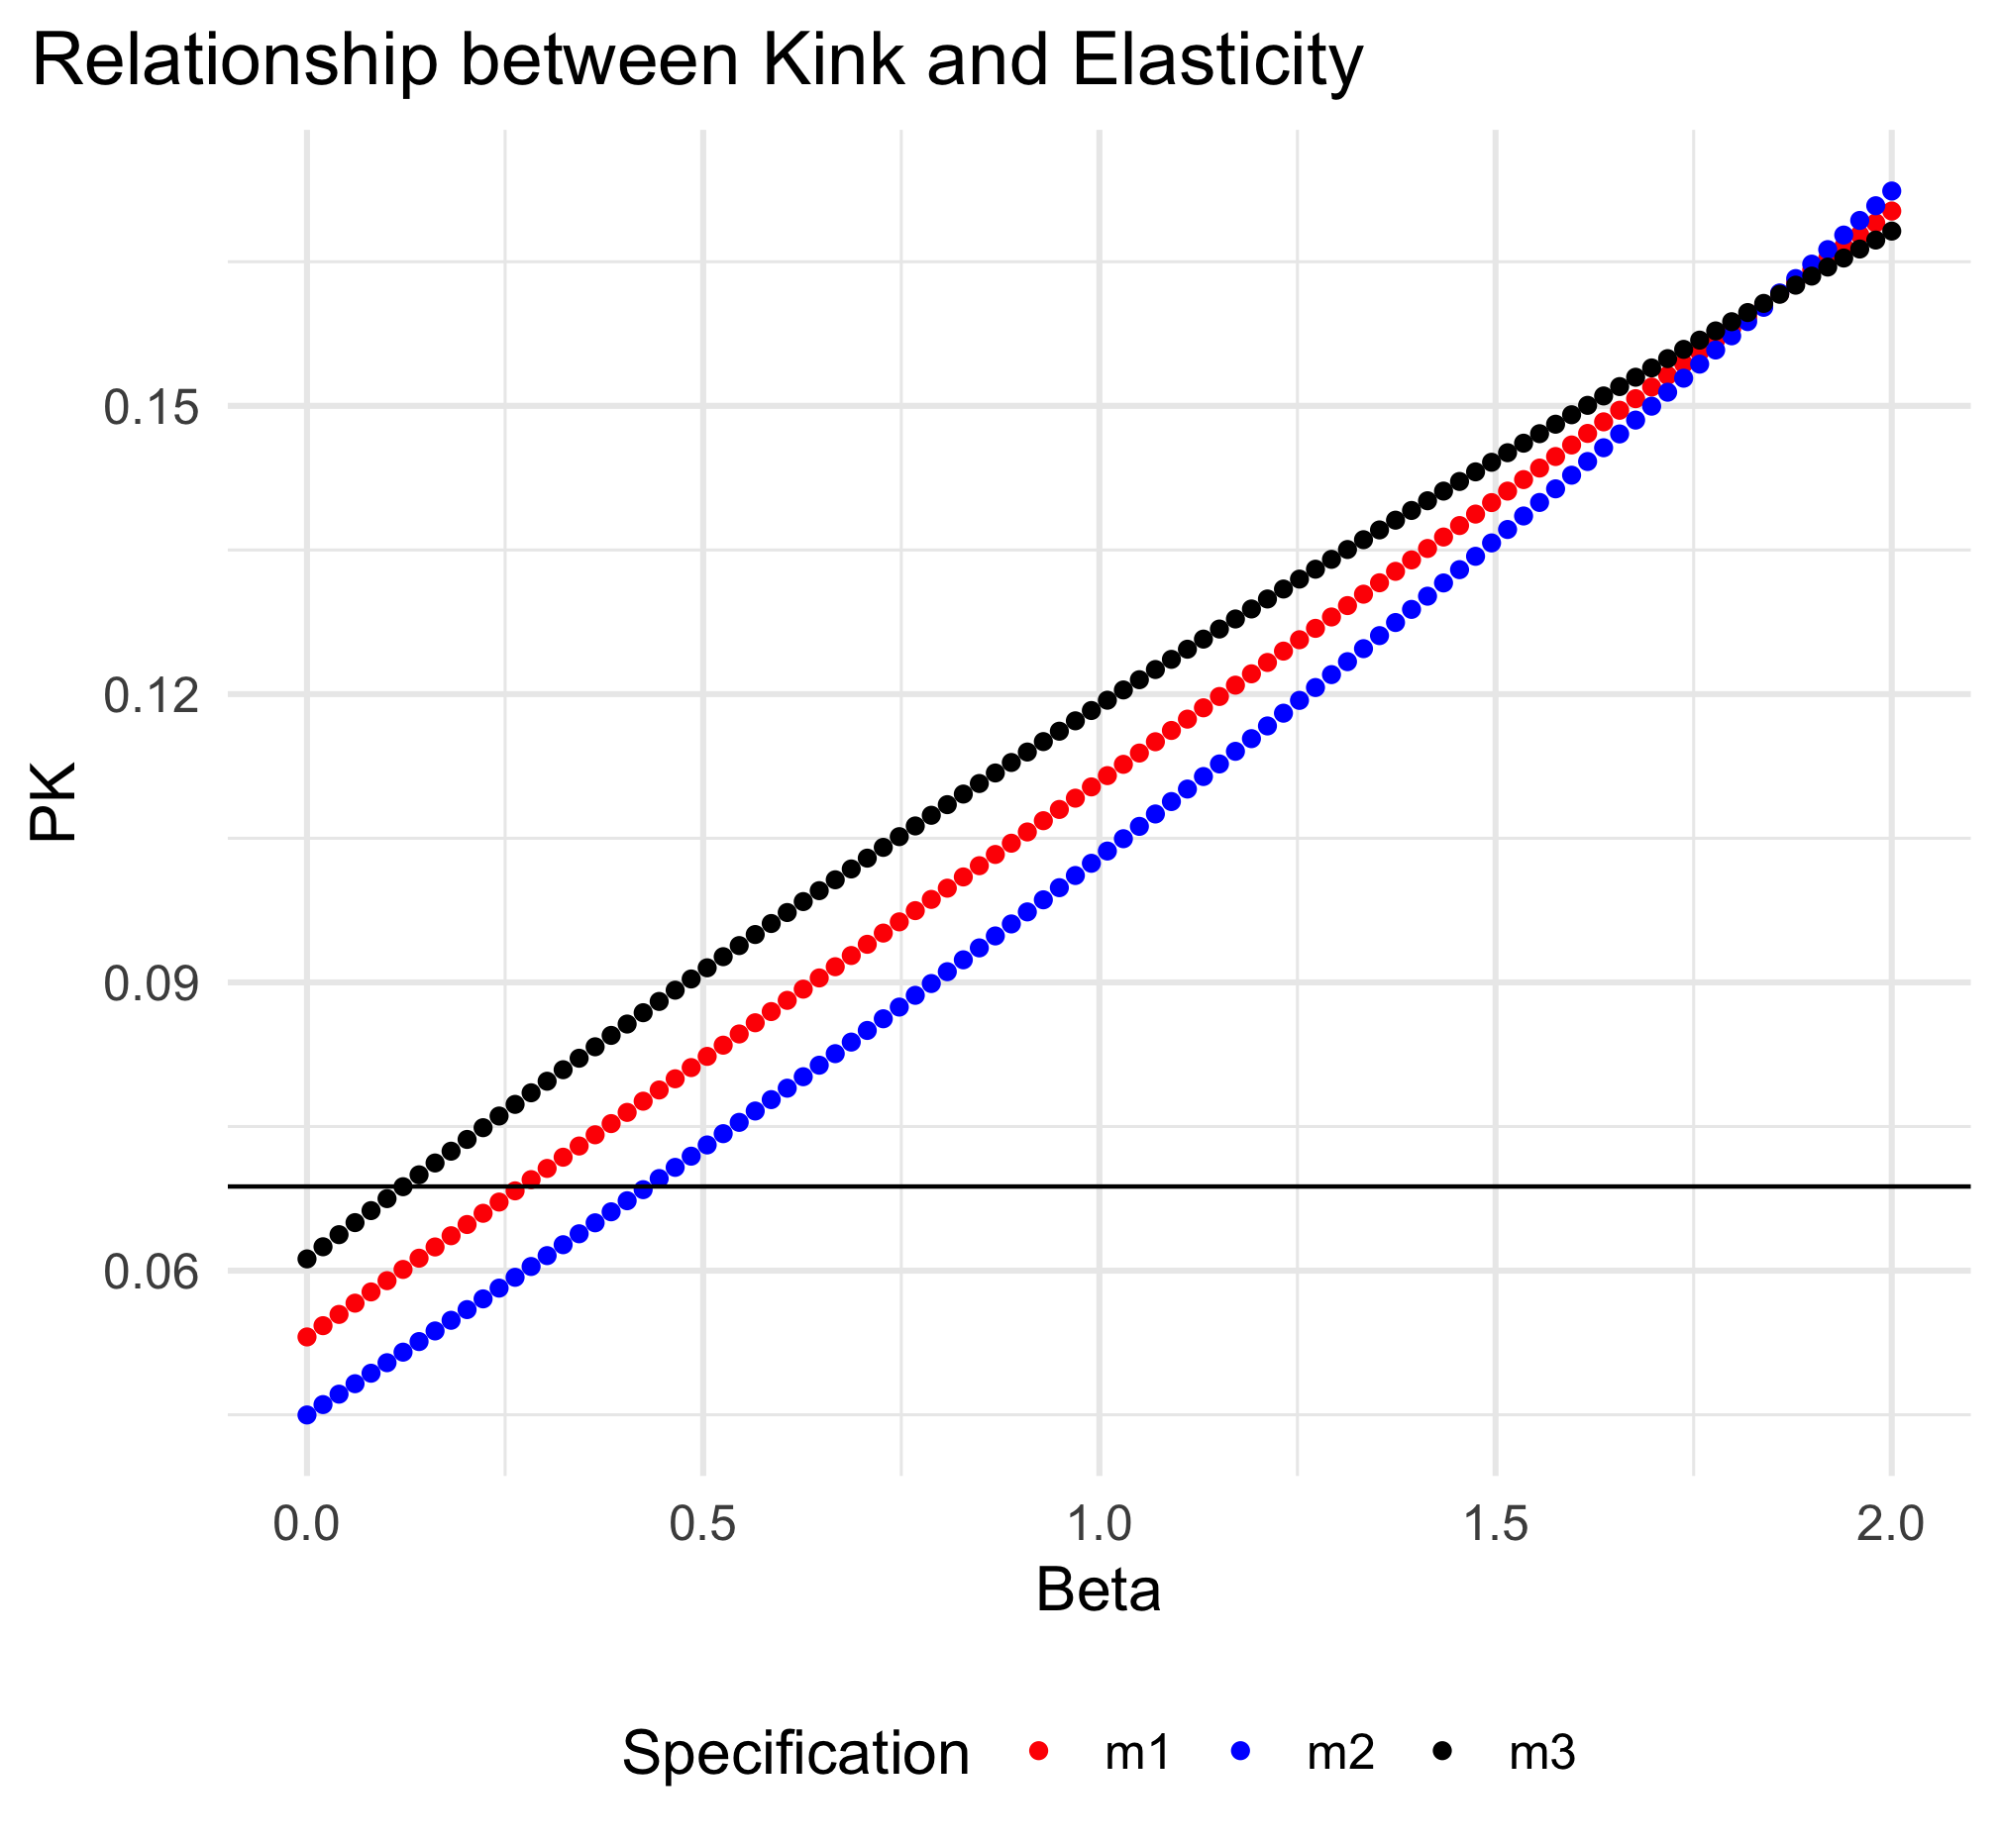
\includegraphics[width=0.75\textwidth]{ps2/4c.png}
\end{figure}

\begin{table}
\centering
\begin{tabular}{|c|c|}
\hline 
Specification & $\beta$\tabularnewline
\hline 
\hline 
1 & 0.270\tabularnewline
\hline 
2 & 0.430\tabularnewline
\hline 
3 & 0.122\tabularnewline
\hline 
\end{tabular}

\caption{Estimated elasticities}
\end{table}


\end{solution}

\pagebreak
\begin{problem}{d}
Compare the magnitudes of these elasticities. How to explain the relationship between them? What can you say about identification of taxable income elasticity based on these results?
\end{problem}
\begin{solution}
As we assume more density towards $\eta_{1}$ we get a higher value
of $\beta$. As we assume more density towards $\eta_{2}$ we get
a lower value of $\beta$. Clearly our estimate of the elasticity
is highly sensitive to our assumptions about the density. 

We can see that $\beta$ is not identified even though $\rho_{2}$
is close to $\rho_{1}$. When $P_{K}$ > 0, we can always find a density
$\phi\left(\eta\right)$ that spits out our chosen $\beta$.
\end{solution}

\begin{problem}{e}
Compute bounds on the taxable income elasticity under the assumption of increasing pref- erences density
\end{problem}
\begin{solution}
Blomquist et. al. 2021 show that since we assume monotonic density, $\sigma=1$. Our non-parametric estimators

$$
D^{-}(\beta)=f^{-}\left(y_{1}\right)\left[y_{2}\left(\frac{\rho_{1}}{\rho_{2}}\right)^{\beta}-y_{1}\right], D^{+}(\beta)=f^{+}\left(y_{2}\right)\left[y_{2}-y_{1}\left(\frac{\rho_{2}}{\rho_{1}}\right)^{\beta}\right] .
$$

So we can estimate the bounds on $\beta$ as follows
\begin{equation}
\begin{aligned}
&\bar{\sigma} \max \left\{\hat{D}^{-}\left(\hat{\beta}_{\ell}\right), \hat{D}^{+}\left(\hat{\beta}_{\ell}\right)\right\}=\widehat{\operatorname{Pr}}\left(y_{1} \leq Y \leq y_{2}\right) = \widehat{P}_K, \\
&\sigma \min \left\{\hat{D}^{-}\left(\hat{\beta}_{u}\right), \hat{D}^{+}\left(\hat{\beta}_{u}\right)\right\}=\widehat{\operatorname{Pr}}\left(y_{1} \leq Y \leq y_{2}\right) = \widehat{P}_K .
\end{aligned}
\end{equation}

\begin{figure}[!htb]
    \centering    
    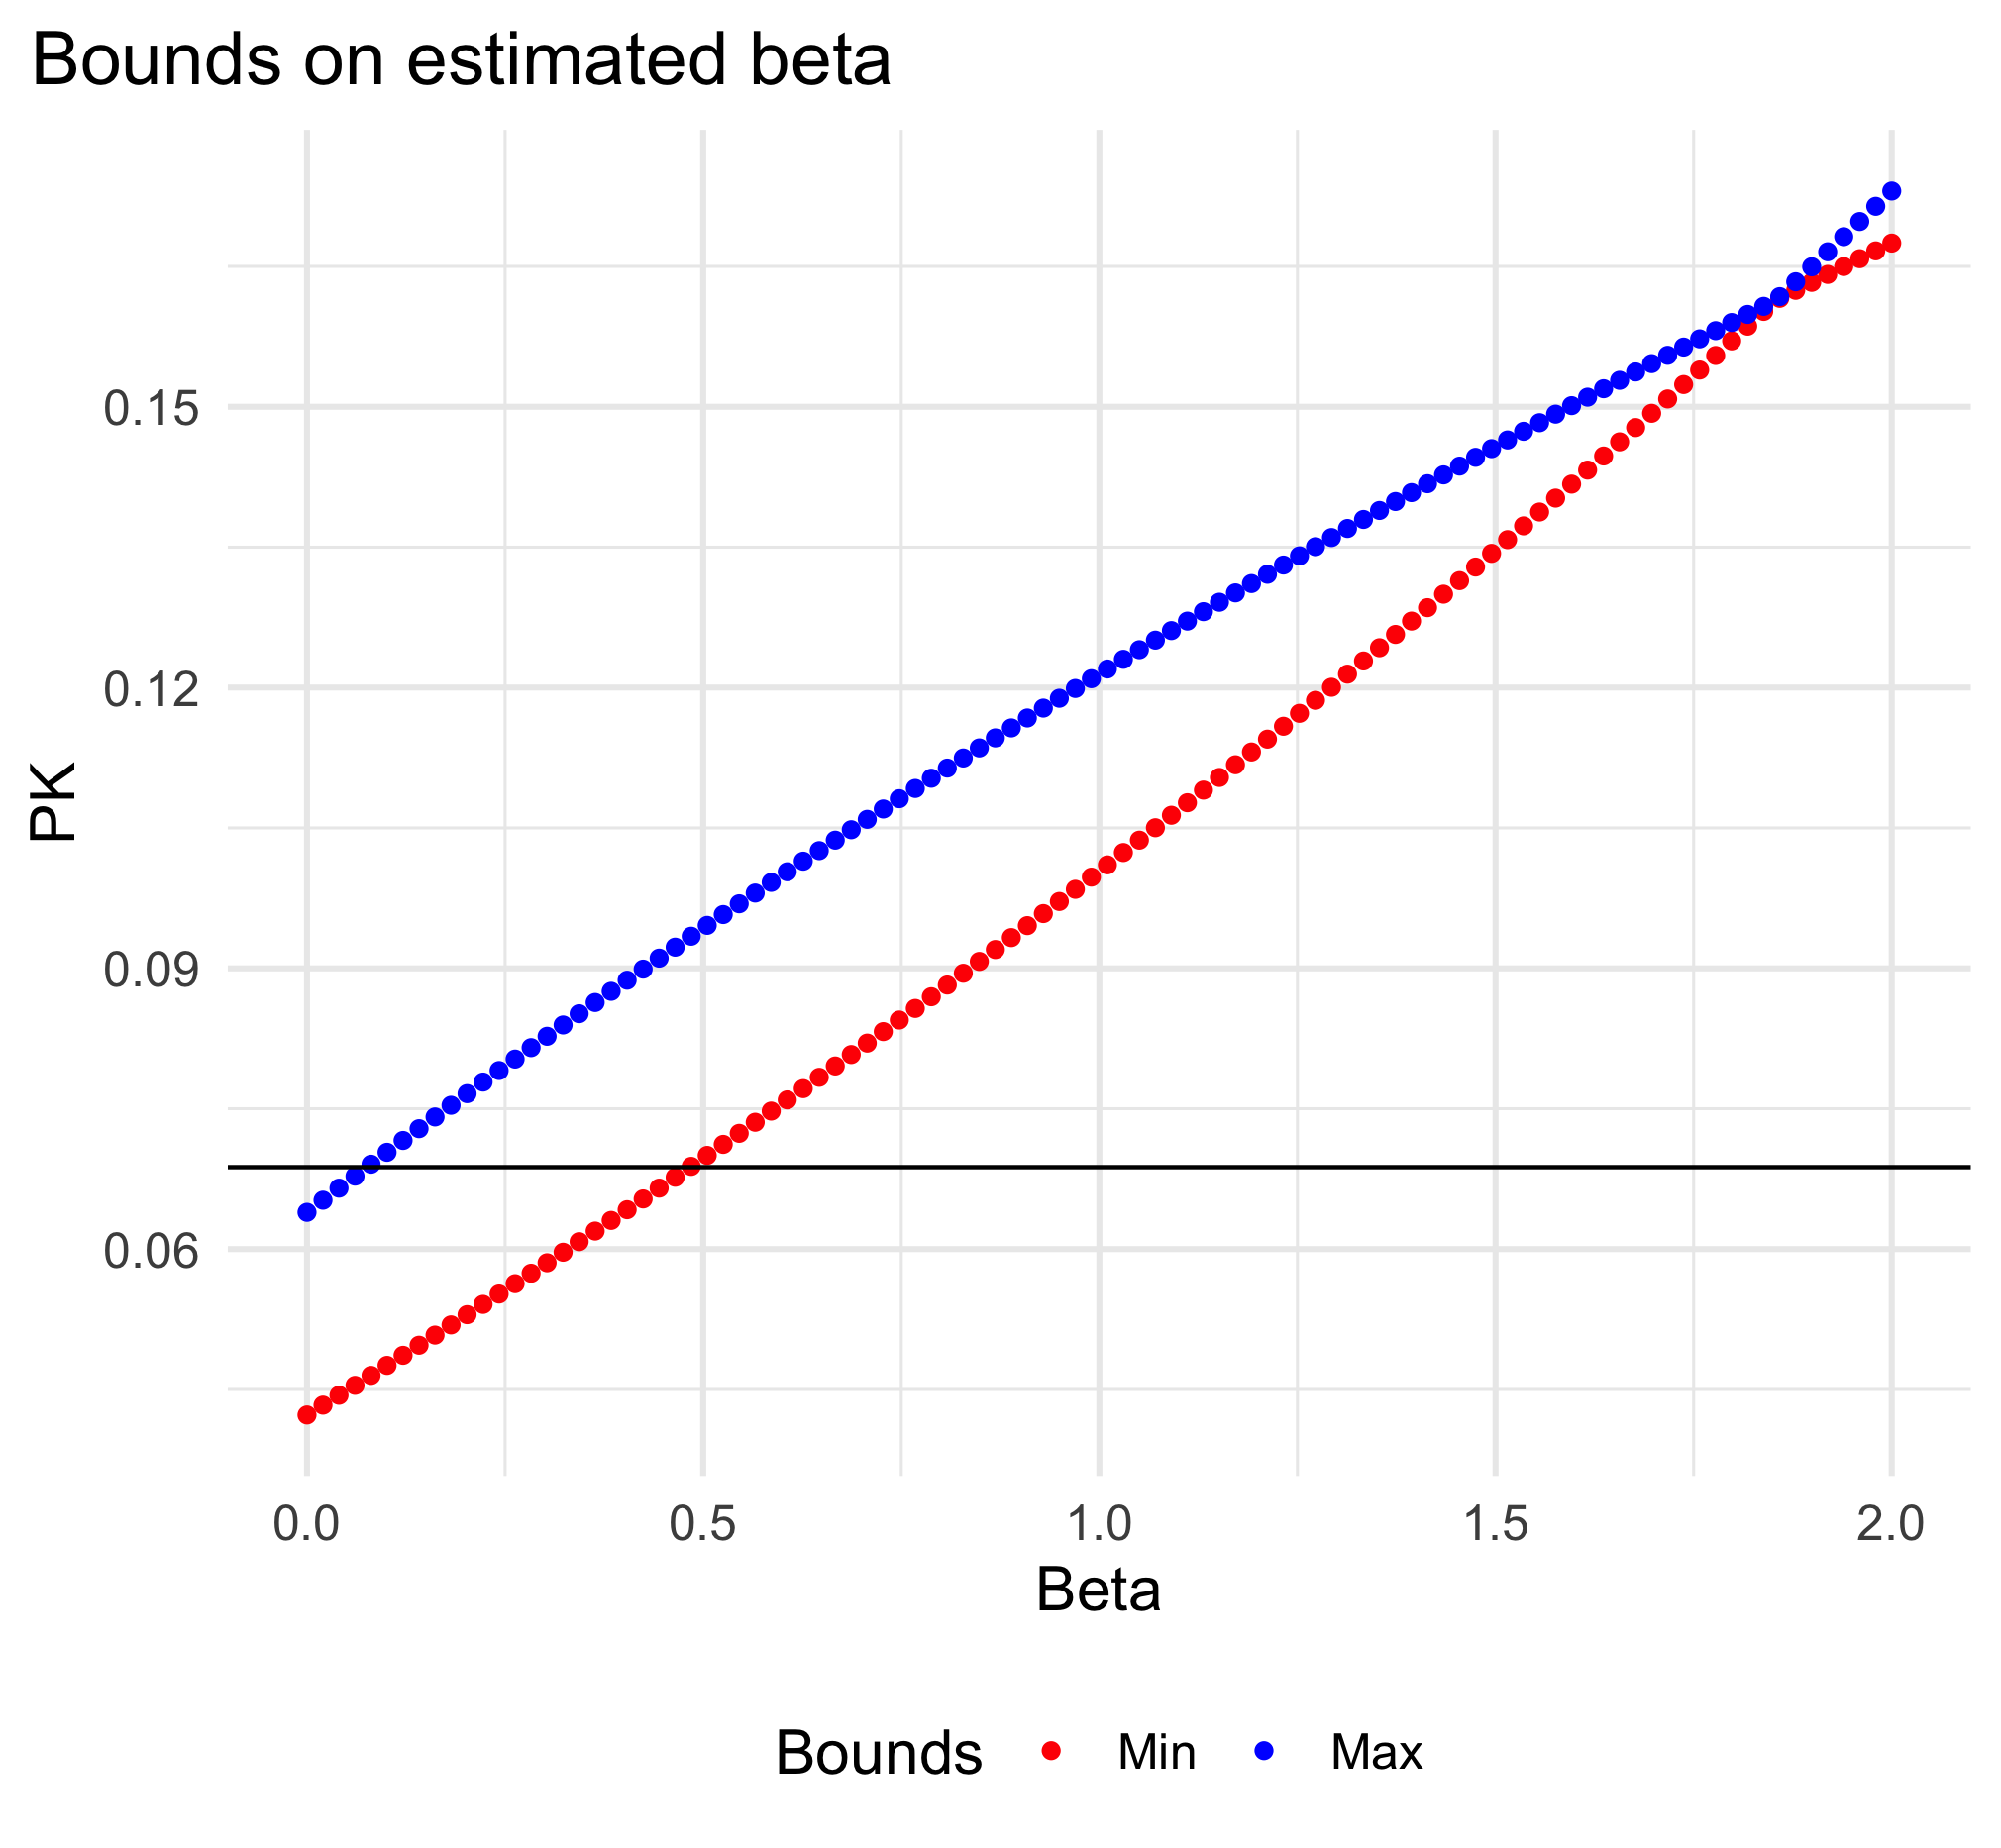
\includegraphics[width=0.75\textwidth]{ps2/4e.png}
\end{figure}



\end{solution}

\begin{problem}{f}
What formal condition on the value of $\beta$ would justify the linearity assumption for the preference density on $\eta_1, \eta_2$. Does the elasticity you computed in c.1 satisfy this condition?
\end{problem}
\begin{solution}
We know from Blomquist (2021) that it is okay to assume that $\phi$
is linear if the kink region is small. In other words, if people only
adjust in a small range then we can approximate the density in that
small range with a linear density. 

However, this is still tricky when it comes to identification. Why?
Because the kink region depends on $\beta$. In the iso-elastic case
we had
\begin{align*}
\begin{bmatrix}\eta_{1} & \eta_{2}\end{bmatrix} & =\begin{bmatrix}K\rho_{1}^{-\beta} & K\rho_{2}^{-\beta}\end{bmatrix}\\
\end{align*}

Clearly the kink region depends on $\beta$. So when Saez (2010) assumes
linear density - justified by the fact that it is within a small kink
region he is assuming that the kink region is small. However we cannot
know if the kink region is small without knowing $\beta$. So assuming
the kink region is small already imposes a restriction on $\beta$.Fundamentally
we have one moment condition and are trying to estimate two things
it is hard. 
\end{solution}

\end{document}
